\chapter{Méthode + Théorie}

\section{Structure d'une protéine et d'un complexe}
\begin{itemize}
  \item Atomes
  \item Interface
  \item .pdb
\end{itemize}

\begin{figure}[ht]
  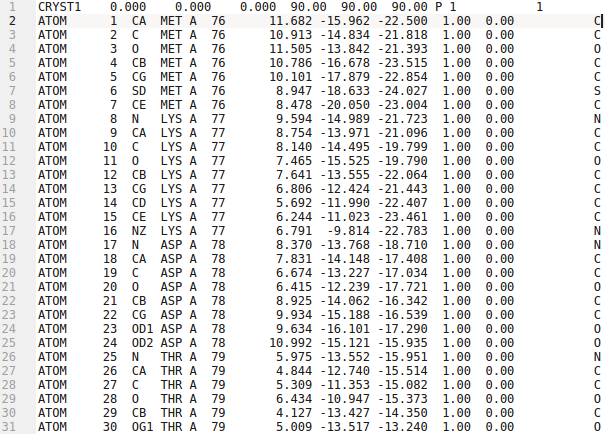
\includegraphics[width=\textwidth]{figures/pdb_example.png}
  \caption{Exemple de fichier .pdb}
  \label{fig::pdb_file}
\end{figure}

\section{Triangulation de Delaunay}
\begin{itemize}
  \item Nuage de points
  \item Explication + schema
  \item Dual : Diagramme de Voronoï
\end{itemize}

\begin{figure}[ht]
\centering
\begin{subfigure}{0.4\textwidth}
  \centering
  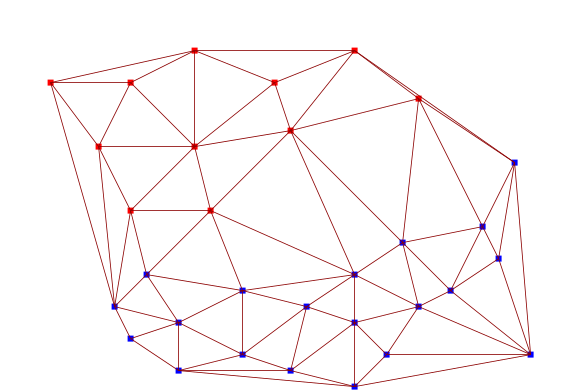
\includegraphics[width=\textwidth]{figures/delaunay.png}
  \caption{Triangulation de Delaunay}
  \label{fig::delaunay_tr}
\end{subfigure}%
\begin{subfigure}{0.2\textwidth}
  \centering
  $\Longrightarrow$
\end{subfigure}%
\begin{subfigure}{0.4\textwidth}
  \centering
  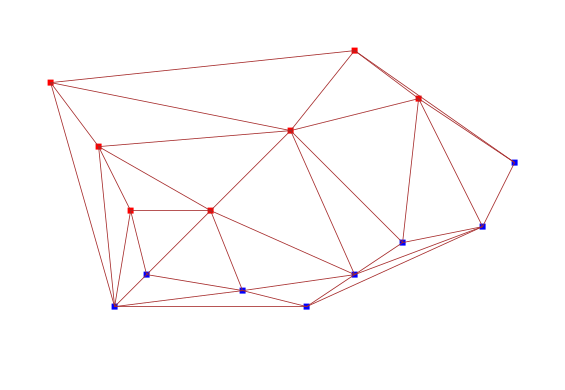
\includegraphics[width=\textwidth]{figures/delaunay_reduced.png}
  \caption{Triangulation réduite}
  \label{fig:delaunay_reduced}
\end{subfigure}
\caption{A figure with two subfigures}
\label{fig:delaunays}
\end{figure}

\begin{figure}[ht]
\centering
\begin{subfigure}{0.45\textwidth}
  \centering
  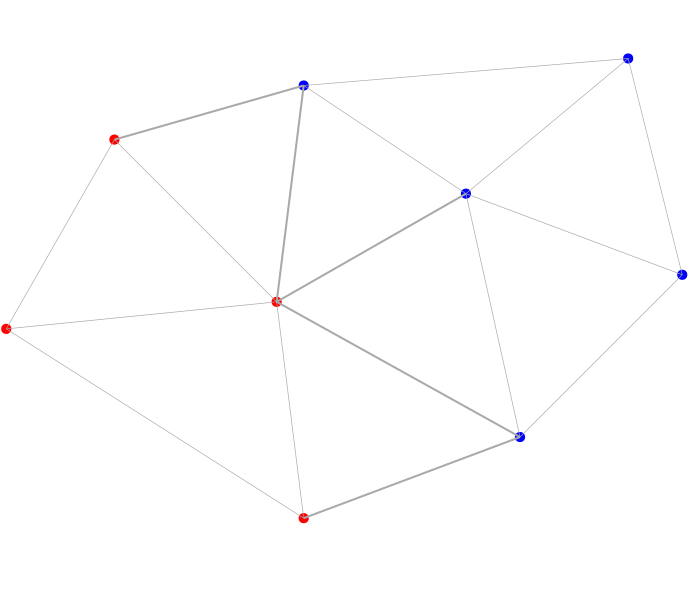
\includegraphics[width=\textwidth]{figures/process_d_1.png}
  \caption{Triangulation de Delaunay}
  \label{fig::process_d_1}
\end{subfigure}%
\begin{subfigure}{0.1\textwidth}
  \centering
  $\Longrightarrow$
\end{subfigure}%
\begin{subfigure}{0.45\textwidth}
  \centering
  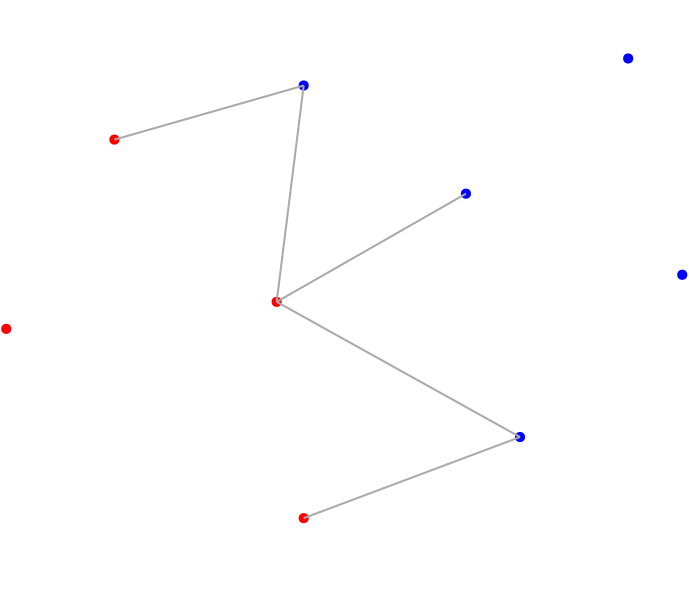
\includegraphics[width=\textwidth]{figures/process_d_2.png}
  \caption{Arêtes à l'interface}
  \label{fig:process_d_2}
\end{subfigure}
\caption{Triangulations et zone utile}
\label{fig:delaunays_process_1}
\end{figure}

\begin{figure}[ht]
\centering
\begin{subfigure}{0.45\textwidth}
  \centering
  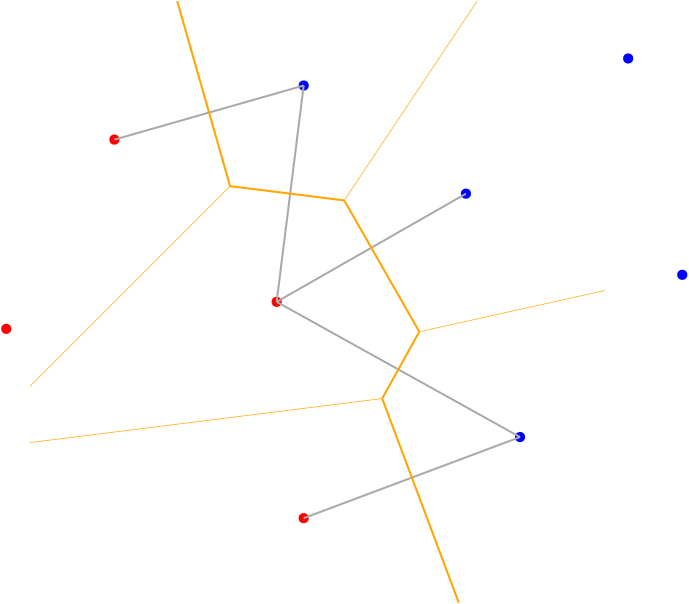
\includegraphics[width=\textwidth]{figures/process_d_3.png}
  \caption{Diagramme de Voronoï}
  \label{fig::process_d_3}
\end{subfigure}%
\begin{subfigure}{0.1\textwidth}
  \centering
  $\Longrightarrow$
\end{subfigure}%
\begin{subfigure}{0.45\textwidth}
  \centering
  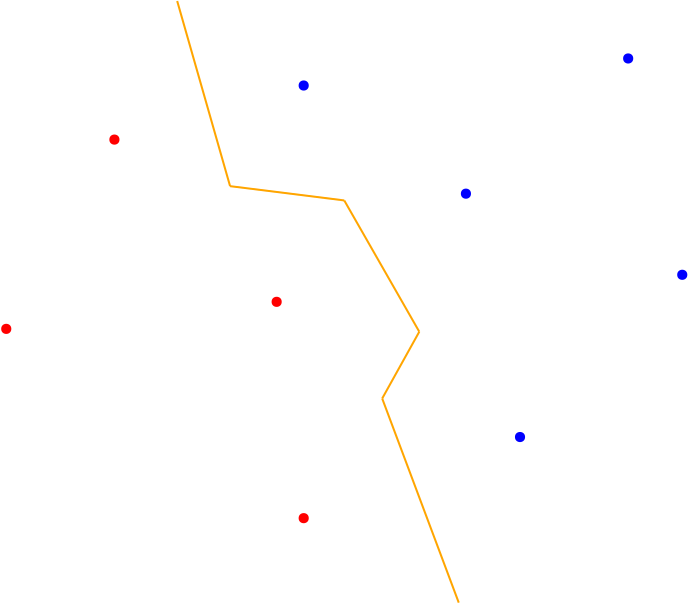
\includegraphics[width=\textwidth]{figures/process_d_4.png}
  \caption{Interface}
  \label{fig:process_d_4}
\end{subfigure}
\caption{Recherche de la surface de contact}
\label{fig:delaunays_process_2}
\end{figure}

\begin{figure}[ht]
  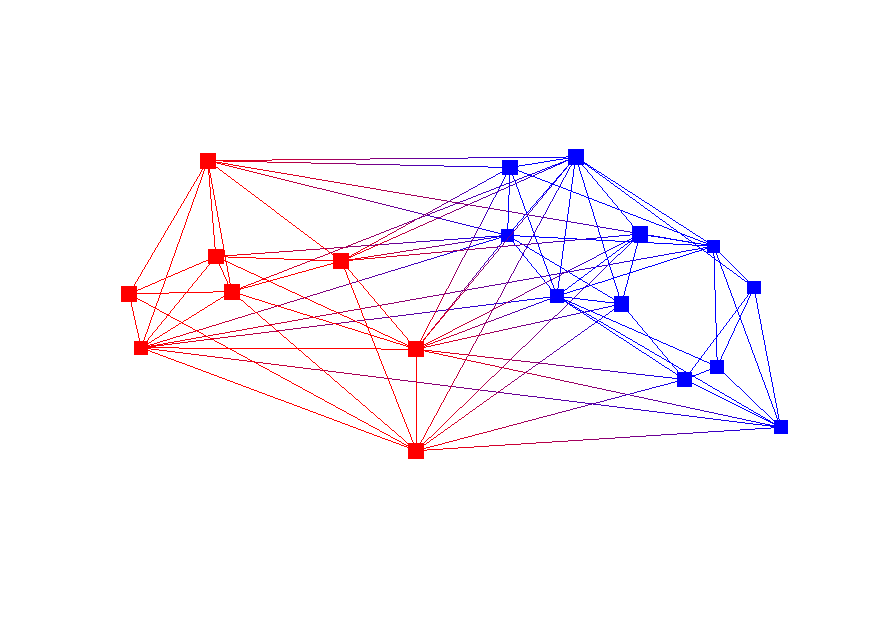
\includegraphics[width=\textwidth]{figures/3d_triangulation.png}
  \caption{Triangulation de Delaunay 3D }
  \label{fig::delaunay_3d}
\end{figure}

\section{CGAL}
\begin{itemize}
  \item Structures
  \item Iterateurs
  \item Compilation $\to$ Cmake
\end{itemize}
